%==================================================
%      PREAMBOLO e DICHIARAZIONI INIZIALI
%==================================================
\documentclass[10pt,oneside,a4paper]{article}

\usepackage[latin1]{inputenc} 
\usepackage[italian]{babel}
\usepackage[T1]{fontenc}
\usepackage{siunitx} %Inserisce automaticamente i dati con le unit�  di misura correttamente formattate del SI (utilizzo: \SI{0.82}{m^2}, in generale \SI{misura con il punto decimale}{unit�  di misura})
\sisetup{output-decimal-marker = {.}, separate-uncertainty = true, input-uncertainty-signs = \pm, detect-weight=true, detect-family=true} %per usare SI con il punto decimale
\usepackage{listings} %Per citare codice informatico formattandolo correttamente
\usepackage{amsmath,amsthm,verbatim,amssymb,amsfonts,amscd,graphicx,mathtools}
\usepackage[makeroom]{cancel}
\newcommand{\abs}[1]{\left\lvert\,#1\,\right\rvert}
\usepackage{geometry}
\usepackage{epigraph}
\usepackage{booktabs}	%tabelle migliorate
\usepackage{tablefootnote}	%note a pi� di pagina in tabella
\usepackage{threeparttable} %tabella con note a pi� di tabella
\usepackage{caption}	%descrizione per figure
\usepackage{dblfnote}
\captionsetup{tableposition=top,figureposition=bottom,font=small} %setup descrizione
\usepackage{float}
\usepackage{esvect} %vettori
\usepackage{longtable} %tabelle lunghe
\usepackage[dvipsnames]{xcolor}
\definecolor{sepia}{HTML}{80002A}
\usepackage[colorlinks=true, citecolor=black, linkcolor=sepia, urlcolor=black]{hyperref}
\usepackage{mathrsfs}
\usepackage{circuitikz}


\usepackage{multicol}
\newenvironment{Figure}
  {\par\medskip\noindent\minipage{\linewidth}}
  {\endminipage\par\medskip}

\newcommand{\var}{\operatorname{var}}
\newcommand{\cov}{\operatorname{cov}}


\usepackage{listings} %Per inserire codice
\lstnewenvironment{codice_c}[1][]
{\lstset{basicstyle=\small\ttfamily, columns=fullflexible,
keywordstyle=\color{red}\bfseries, commentstyle=\color{blue},
language=C, basicstyle=\small,
numbers=left, numberstyle=\tiny,
stepnumber=2, numbersep=5pt, frame=shadowbox,  showstringspaces=false, #1}}{}

%==================================================
%                  PRIMA PAGINA
%==================================================

\title{\textsc{\textbf{Esercitazione 3}: Amplificatore operazionale 1}}
\author{\small{G. Galbato Muscio} \and \small{L. Gravina} \and \small{L. Graziotto}}
\date{\today}

\begin{document}
	\begin{figure}
		\centering
		
\includegraphics[scale=0.5, trim={2.8cm 8.9cm 0 9cm}, clip]{logo.png}
	\end{figure}
	\maketitle
	\begin{center} 
		\fbox{{\fontsize{12pt}{8mm}\textsc{Gruppo 11}}} \\
	\end{center}
\hrule
\vspace{0.5cm}
\renewcommand{\abstractname}{Abstract}
\begin{abstract}
Si misurano lo \emph{slew rate} e il prodotto guadagno per banda passante di un amplificatore operazionale LM358. Quindi, lo si utilizza per realizzare un circuito derivatore.
\end{abstract}
\vspace{4cm}
\tableofcontents %Indice
\newpage


\pagebreak
\begin{multicols}{2}
%==================================================
%      		MISURA DELLO SLEW RATE
%==================================================
\section{Misura dello \emph{slew rate}}
Si utilizza nel seguito l'amplificatore operazionale LM358, e lo si alimenta con una differenza di potenziale di $\pm \SI{12}{V}$, connettendo gli ingressi \texttt{V+} e \texttt{GND} alla doppia alimentazione in continua, positiva e negativa. 

Si realizza, per ottimizzare la misura dello \emph{slew rate}, un \emph{emitter follower}, ossia un amplificatore non invertente con amplificazione unitaria, illustrato nel circuito seguente.

\begin{center}
\begin{circuitikz}
\draw (0,0) node[op amp, yscale=-1] (opamp) {}
(opamp.+) to[short, -*] ++(-0.75,0) node[left] {$V_\text{i}$}
(opamp.-) to[short] ++(0, -1.25) -| (opamp.out)
(opamp.out) to[short, *-*] ++(0.5,0) node[right] {$V_\text{o}$}
;\end{circuitikz}
\end{center}

Si invia all'ingresso non invertente dell'op-amp un segnale rettangolare (onda quadra) di frequenza \SI{5.4 \pm 0.2}{kHz} e ampiezza variabile, oscillante tra $0$ e $V_i$. Osservando sull'oscilloscopio il segnale in uscita, si osserva che l'amplificazione � effettivamente circa unitaria (si ha $A_v = \SI{0.99 \pm 0.03}{}$, con incertezza data dalla misura con l'oscilloscopio), ma la risposta presenta un tempo di salita, ovvero non segue istantaneamente l'ingresso. Selezionando la regione crescente lineare e misurandone la pendenza mediante i cursori, si ricava in ciascun caso la \emph{slew rate} come
\[
S = \frac{\Delta V}{\Delta t} = \frac{V_o}{\Delta t}.
\]
Si riportano in tabella~\ref{tab:slewrate} i valori di $V_i$, di $\Delta V$, di $\Delta t$ e della stima di $S$.

\begin{center}
\captionof{table}{Valori misurati per la stima dello \emph{slew rate}}
\label{tab:slewrate}
\begin{tabular}{c|c|c|c}
\hline
   $V_i$ [V] &   $\Delta t$ [$\mu s$] &   $\Delta V$ [V] &   $S$ [V/$\mu s$] \\
\hline
         6.0 &                 19.4 &              5.8 &             0.301 \\
         4.0 &                 13.4 &              3.7 &             0.279 \\
         5.0 &                 16.6 &              4.9 &             0.294 \\
         7.2 &                 24.4 &              7.4 &             0.302 \\
         8.7 &                 30.4 &              8.9 &             0.292 \\
\hline
\end{tabular}
\end{center}

La stima dello \emph{slew rate}, data dalla media dei valori misurati con errore associato la deviazione standard, risulta essere
\[
S = \SI{0.294 \pm 0.008}{V / \micro s};
\]
si confronta tale valore con quello dichiarato dal costruttore, di \SI{0.5}{V / \micro s}, che tuttavia � stato calcolato mediante un circuito diverso da quello qui utilizzato. A titolo esemplificativo, si riporta in figura~\ref{fig:slewrate} un'istantanea dell'oscilloscopio, dalla quale risulta visibile il tempo finito impiegato dalla risposta a raggiungere il valore a regime.

\begin{figure}[H]
	\begin{center}
	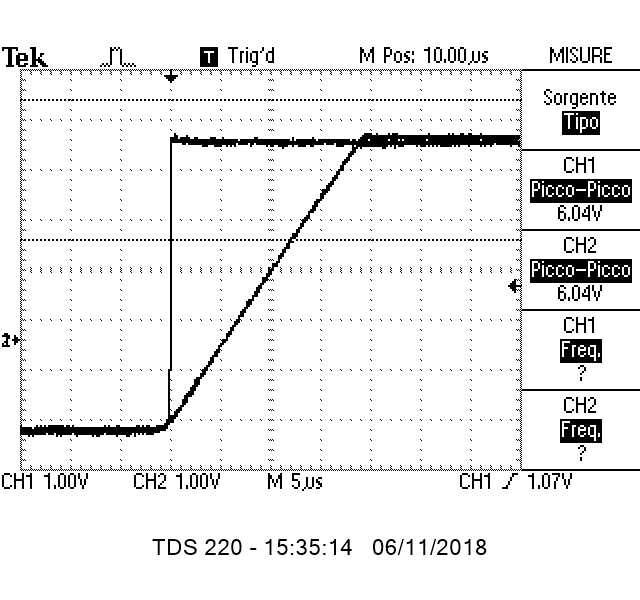
\includegraphics[width=\linewidth]{slew.png}
	\caption{Stima dello \emph{slew rate} utilizzando un'onda quadra}
	\label{fig:slewrate}
	\end{center}
\end{figure}

Si ripete quindi la misura inviando all'ingresso non invertente un segnale sinusoidale del tipo $V_i = V_p \sin(\omega t)$, di frequenza variabile e ampiezza picco-picco $V_p = \SI{7.1 \pm 0.2}{V}$. Si stima anche in questo caso lo \emph{slew rate} variando la frequenza finch� non si veda un segnale in uscita distorto, a $f_D = \SI{13.2 \pm 0.4}{kHz}$; poich� per evitare di vedere un segnale distorto si dovrebbe rispettare la relazione
\[
S \geq A_v V_p 2\pi f,
\]   
si ha che, dalla frequenza a cui si ha il passaggio alla distorsione, si ricava $S = \SI{0.59 \pm 0.02}{V / \micro s}$. Questo valore risulta essere poco accurato (molto meno di quanto lo sia la stima precedente), proprio perch� la stima di dove il segnale cominci ad apparire distorto � soggettiva, e non riproducibile. 


Poich� la banda passante � in questo caso di \SI{1}{MHz}, come dichiarato dal costruttore, e l'amplificazione � unitaria, si ha che � verificata la richiesta di lavorare sotto la frequenza di taglio. 

%==================================================
%    MISURA DEL PRODOTTO GUADAGNO-BANDA PASSANTE
%==================================================
\section{Misura del prodotto guadagno per banda passante}
Si costruisce un amplificatore invertente con medesima alimentazione della sezione precedente ($\pm$\SI{12}{V}) e se ne misura la risposta in funzione della frequenza, per vari valori dell'amplificazione, ottenuti cambiando le resistenze della rete di reazione negativa, ricordando che in questo caso
\[
A_v = -\frac{R'}{R}.
\]
Il circuito utilizzato � il seguente.

\begin{center}
\begin{circuitikz}
\draw (0,0) node[op amp] (opamp) {}
(opamp.+) -| ++(-0.5,-0.5) node[ground]{}
(opamp.out) to[short, *-*] ++(0.5,0) node[right] {$V_\text{o}$}
(opamp.-) to[short] ++(-0.25,0) to[R=$R$] ++(-1.5,0) node[] (Vs) {} ++(0,-2) node[] (ground) {}
(ground) node[ground] {} to[sV = $V_s$, invert] (Vs)
(opamp.-) -| ++(0,1) to[R = $R'$] ++(1.5,0) -| (opamp.out)
(opamp.-) node[circ] {}
;\end{circuitikz}
\end{center}

Le resistenze vengono scelte tenendo conto che si vuole minimizzare la corrente che scorre all'interno dell'OP-AMP (poich� non si ha a che fare con il caso ideale), e che si vuole ottenere una resistenza di ingresso di valore elevato, in modo da avvicinarsi al caso ideale. 

Si invia in ingresso al circuito un segnale sinusoidale di ampiezza picco-picco $V_s$, in modo che sia rispettata la disuguaglianza
\[
V_s \leq \frac{S}{2\pi f A} \simeq \SI{80}{mV},
\]
utilizzando i dati forniti dal costruttore, al fine di evitare un segnale distorto in $V_o$. Sui canali \texttt{CH1} e \texttt{CH2} dell'oscilloscopio vengono verificati rispettivamente il segnale di ingresso e di uscita, e si verifica che quest'ultimo � sfasato di circa $\pi$ rispetto al primo, come previsto dalla dinamica dell'amplificatore invertente.

Si riportano nella tabelle~\ref{tab:gainbandwidthR1}, \ref{tab:gainbandwidthR2}, \ref{tab:gainbandwidthR3}, \ref{tab:gainbandwidthR4} in appendice i valori di $V_s$, $V_o$, dell'amplificazione $A_v = V_o / V_s$ e della frequenza a cui viene effettuata la misura $f$ per i diversi valori delle resistenze $R$ e $R'$ con le quali viene realizzata la rete di reazione. Tali resistenze sono misurate con il multimetro, mentre le tensioni e le frequenze con l'oscilloscopio. In figura~\ref{fig:bodeGainbandwidth} � riportato il diagramma di Bode con i punti sperimentali; da questo si ricava il guadagno come media dei valori dell'amplificazione nella regione dove essa � costante, con associata l'incertezza data dall'oscilloscopio (dell'ordine del $3\%$), che risulta dominante rispetto a quella statistica, mentre la banda passante � stimata dall'ascissa del punto di intersezione tra la retta che rappresenta la discesa dell'amplificazione dopo la frequenza di taglio (ottenuta interpolando linearmente i dati) con la retta orizzontale relativa ad un'amplificazione di \SI{-3}{dB}, che rappresenta appunto il valore di $A_v$ alla frequenza di taglio. Si verifica inoltre che la pendenza della retta decrescente sia compatibile con il valore di \SI{-20}{dB/dec}.

\begin{figure}[H]
	\begin{center}
	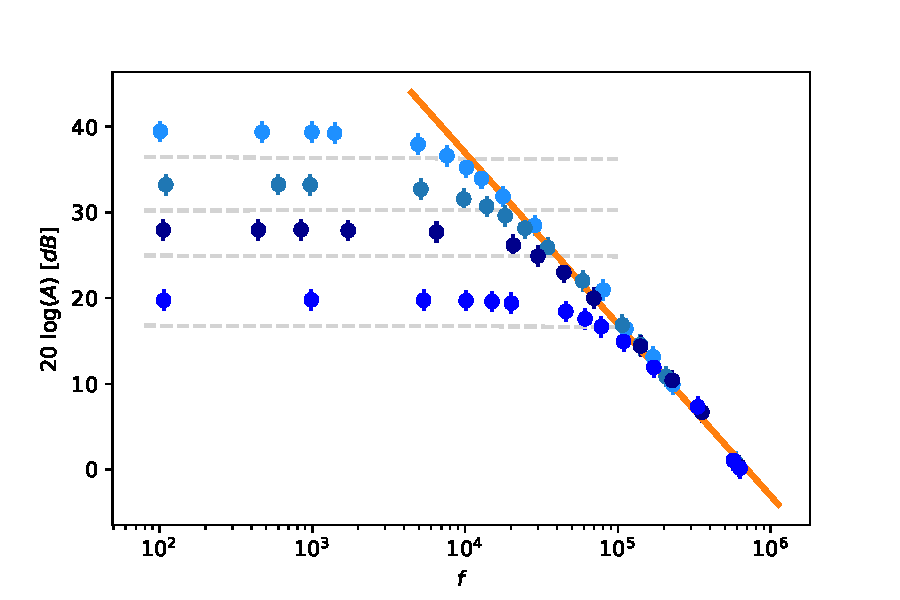
\includegraphics[width=\linewidth]{banda.pdf}
	\caption{Diagramma di Bode per la misura del prodotto guadagno per banda passante}
	\label{fig:bodeGainbandwidth}
	\end{center}
\end{figure}

Per le differenti configurazioni della rete di reazione, si ottengono i valori riportati in tabella~\ref{tab:riepilogoGainbandwidth}.

\begin{center}
\captionof{table}{Prodotto guadagno per banda passante per le diverse reti di reazione}
\label{tab:riepilogoGainbandwidth}
\begin{tabular}{c|c|c|c}
\hline
   $V_i$ [V] &   $\Delta t$ [$\mu s$] &   $\Delta V$ [V] &   $S$ [V/$\mu s$] \\
\hline
        6.04 &                 19.4 &             5.84 &             0.301 \\
        3.96 &                 13.4 &             3.74 &             0.279 \\
        5.00 &                 16.6 &             4.88 &             0.294 \\
        7.20 &                 24.4 &             7.36 &             0.302 \\
        8.72 &                 30.4 &             8.88 &             0.292 \\
\hline
\end{tabular}
\end{center}

Si ottiene una stima conclusiva del prodotto guadagno per banda passante, data dalla media pesata delle differenti misurazioni, di 
\[
\text{GBW product} = \SI{111 \pm 111}{kHz},
\]
compatibile con il valore atteso di \SI{1}{MHz} riportato nel datasheet.

%==================================================
%    			CIRCUITO DERIVATORE
%==================================================
\section{Circuito derivatore}
Si realizza un circuito derivatore con opportuna scelta delle componenti $R_1$ e $C$ affinch� si abbia un $\tau = R_1 C$ dell'ordine di $10^{-4}$ \SI{}{s}. Si sceglie la resistenza $R_2$, inoltre, in modo tale che sia $R_2 C \ll R_1 C$. Il circuito utilizzato � il seguente.

\begin{center}
\begin{circuitikz}
\draw (0,0) node[op amp] (opamp) {}
(opamp.+) -| ++(-0.5,-0.5) node[ground]{}
(opamp.out) to[short, *-*] ++(0.5,0) node[right] {$V_\text{o}$}
(opamp.-) to[short] ++(-0.25,0) to[C=$C$] ++(-1,0) to[R=$R_2$] ++(-1.5,0) node[circ] {} node[left] {$V_s$} 
(opamp.-) -| ++(0,1) to[R = $R_1$] ++(1.5,0) -| (opamp.out)
(opamp.-) node[circ] {}
;\end{circuitikz}
\end{center}

L'OP-AMP � alimentato ancora con una tensione di $\pm$ \SI{12}{V}; i valori delle resistenze e della capacit� sono
\[
\begin{aligned}
R_1 &= \SI{99.2 \pm 0.5}{k\ohm} \\
R_2 &= \SI{2.17 \pm 0.01}{k\ohm} \\
C &= \SI{1.005 \pm 0.005}{\nano F},
\end{aligned}
\]
misurati con il multimetro e con il ponte. Si fornisce all'ingresso invertente dell'amplificatore un'onda quadra di ampiezza picco-picco $V_s = \SI{40 \pm 1.2}{mV}$ e frequenza $f = \SI{1.97 \pm 0.06}{kHz}$, e si osserva al \texttt{CH2} dell'oscilloscopio una $V_o$ impulsiva, localizzata dove si ha il passaggio dell'onda dalla tensione massima a quella minima; si riporta in figura~\ref{fig:derivatoreOndaquadra} un'istantanea dell'oscilloscopio per questa configurazione.

\begin{figure}[H]
	\begin{center}
	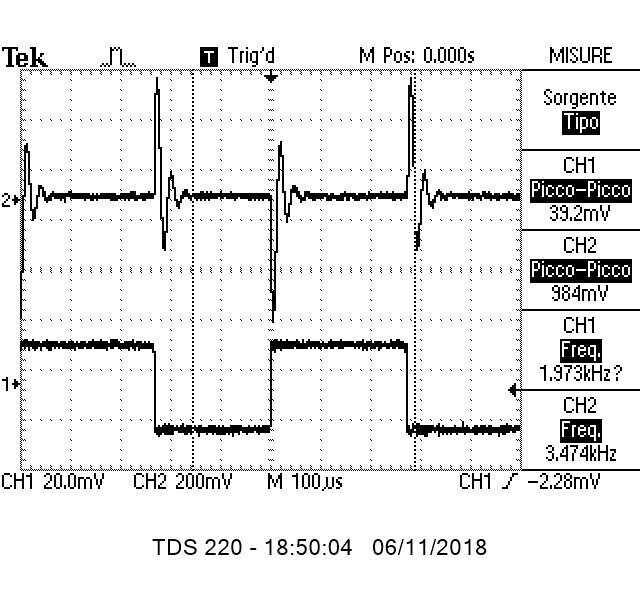
\includegraphics[width=\linewidth]{delta.png}
	\caption{Screenshot dell'oscilloscopio per l'onda quadra in ingresso al derivatore}
	\label{fig:derivatoreOndaquadra}
	\end{center}
\end{figure}

\begin{figure}[H]
	\begin{center}
	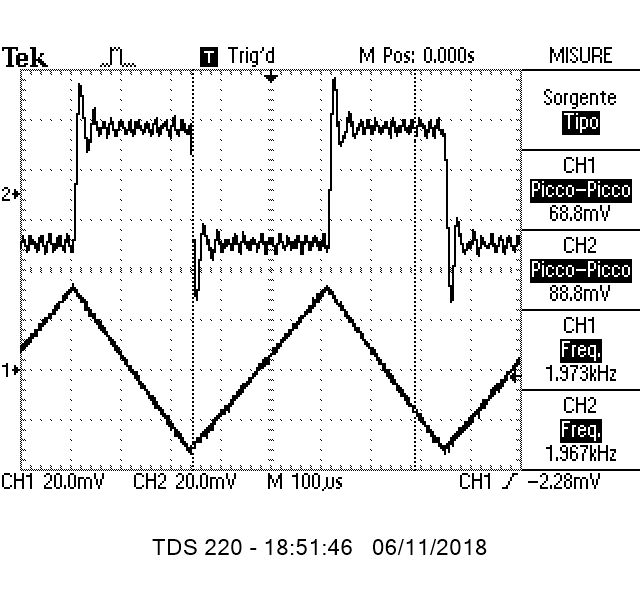
\includegraphics[width=\linewidth]{triangolare.png}
	\caption{Screenshot dell'oscilloscopio per l'onda quadra in ingresso al derivatore}
	\label{fig:derivatoreTriangolare}
	\end{center}
\end{figure}

Si invia inoltre come segnale in ingresso un'onda triangolare di frequenza \SI{1.90 \pm 0.06}{kHz} di ampiezza picco-picco \SI{66 \pm 2}{mV}. Si osserva in uscita (e si riporta un'istantanea dell'oscilloscopio in figura~\ref{fig:derivatoreTriangolare}) un'onda quadra (che presenta tuttavia degli impulsi nei punti corrispondenti ai vertici dell'onda triangolare) di ampiezza \SI{46.4 \pm 1.3}{mV}. Si misura con i cursori la pendenza dei tratti in salita e in discesa dell'onda triangolare, $\Delta V / \Delta t$ ottenendo rispettivamente \SI{244 \pm 10}{V/s} e \SI{-281 \pm 11}{V/s}. 



Si studia quindi la risposta in frequenza, inviando un segnale sinusoidale di ampiezza picco-picco $V_s$ e frequenza $f$, e misurando con l'oscilloscopio l'ampiezza $V_o$, quindi si ricava l'amplificazione $A_v = V_o / V_s$. Si riportano nella tabella~\ref{tab:derivatore} in appendice le diverse misure, e nella figura~\ref{fig:bodeDerivatore} il diagramma di Bode dei dati sperimentali. Si osserva, come previsto, che il comportamento del derivatore reale si discosta da quello ideale a causa del taglio dell'amplificazione alle alte frequenze. Si stima la discesa oltre la frequenza di taglio mediante interpolazione lineare, ottenendo una pendenza di \SI{111 \pm 111}{dB/dec}, in accordo con il valore teorico di \SI{-20}{dB/dec}. Per la regione crescente si stima una pendenza di \SI{111 \pm 111}{dB/dec}; poich� in questa si ha che il derivatore realizzato con l'OP-AMP segue l'andamento ideale
\[
\abs{A_v} = \frac{\abs{V_o}}{\abs{V_s}} = R_1 C \omega, 
\]
si confronta tale pendenza con il valore previsto di \SI{20}{dB/dec} e l'intercetta con l'asse delle ascisse, che dal diagramma di Bode � in corrispondenza di $f_0 = \SI{111 \pm 111}{Hz}$, con il valore previsto di $f_0 = 1/ (2\pi R_1 C)$.
\begin{figure}[H]
	\begin{center}
	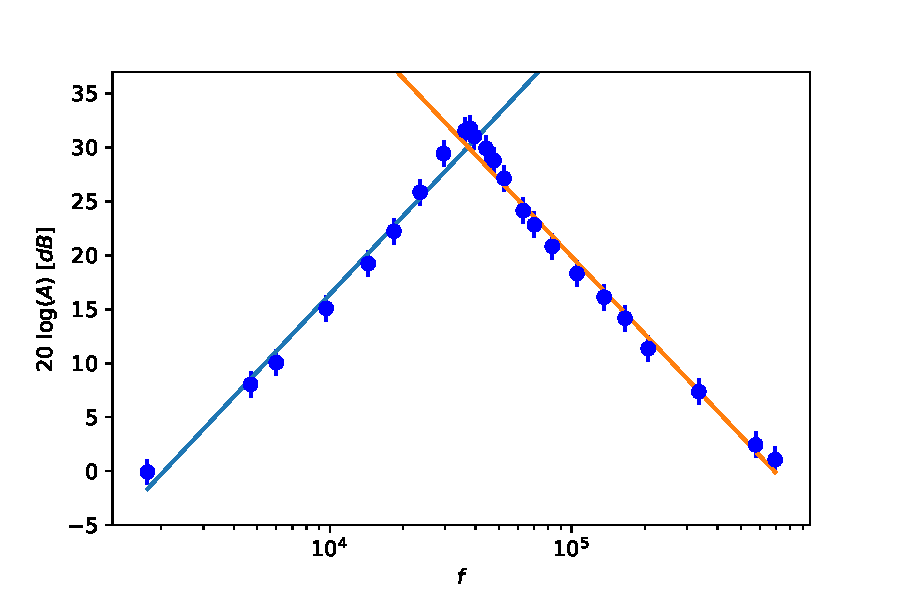
\includegraphics[width=\linewidth]{derivatore.pdf}
	\caption{Screenshot dell'oscilloscopio per l'onda quadra in ingresso al derivatore}
	\label{fig:bodeDerivatore}
	\end{center}
\end{figure}

Si osserva che il passaggio dalla regione crescente a quella decrescente � molto piccato: questo � conseguente alla scelta di $R_2$ molto minore di $R_1$, che permette di approssimare meglio il circuito derivatore al caso ideale, per frequenze inferiori a quella di taglio. 



\end{multicols}
%==================================================
%      				APPENDICE	
%==================================================
\pagebreak
\section{Appendice}

\begin{table}[H]
\begin{center}
\captionof{table}{Misure per la stima del prodotto guadagno per banda passante con resistenza $R' = \SI{1.005 \pm 0.005}{\kilo \Omega}$}
\label{tab:gainbandwidthR1}
\begin{tabular}{c|c|c|c}
\hline
   $f$ [kHz] &   $V_s$ [mV] &   $Vo$ [V] &   $A_v$  \\
\hline
  1.013e+02 &     4.04e+01 &    3.8e+00 &     94.1 \\
  4.700e+02 &     4.10e+01 &    3.8e+00 &     93.2 \\
  9.950e+02 &     4.08e+01 &    3.8e+00 &     93.1 \\
  1.400e+03 &     4.14e+01 &    3.8e+00 &     91.8 \\
  4.930e+03 &     4.20e+01 &    3.3e+00 &     79.0 \\
  7.600e+03 &     4.22e+01 &    2.9e+00 &     67.8 \\
  1.020e+04 &     4.25e+01 &    2.5e+00 &     57.9 \\
  1.280e+04 &     4.24e+01 &    2.1e+00 &     50.0 \\
  1.770e+04 &     4.28e+01 &    1.7e+00 &     39.3 \\
  2.850e+04 &     4.30e+01 &    1.1e+00 &     26.5 \\
  8.000e+04 &     4.30e+01 &    4.8e-01 &     11.2 \\
  1.130e+05 &     4.35e+01 &    2.9e-01 &      6.6 \\
  1.700e+05 &     4.36e+01 &    2.0e-01 &      4.5 \\
  2.290e+05 &     6.76e+01 &    2.1e-01 &      3.1 \\
  5.900e+05 &     7.20e+01 &    8.0e-02 &      1.1 \\
\hline
\end{tabular}
\end{center}
\end{table}

\begin{table}[H]
\begin{center}
\captionof{table}{Misure per la stima del prodotto guadagno per banda passante con resistenza $R' = \SI{2.17 \pm 0.01}{\kilo \Omega}$}
\label{tab:gainbandwidthR2}
\begin{tabular}{c|c|c|c}
\hline
   $f$ [kHz] &   $V_s$ [mV] &   $Vo$ [V] &   $A_v$  \\
\hline
  1.100e+02 &     3.84e+01 &    1.8e+00 &     45.8 \\
  6.000e+02 &     3.82e+01 &    1.8e+00 &     46.1 \\
  9.700e+02 &     3.84e+01 &    1.8e+00 &     45.8 \\
  5.140e+03 &     4.02e+01 &    1.7e+00 &     43.3 \\
  9.800e+03 &     3.88e+01 &    1.5e+00 &     37.9 \\
  1.385e+04 &     3.90e+01 &    1.3e+00 &     34.4 \\
  1.830e+04 &     3.90e+01 &    1.2e+00 &     30.3 \\
  2.465e+04 &     3.90e+01 &    1.0e+00 &     25.6 \\
  3.470e+04 &     3.94e+01 &    7.8e-01 &     19.7 \\
  5.880e+04 &     3.96e+01 &    5.0e-01 &     12.6 \\
  1.070e+05 &     3.96e+01 &    2.8e-01 &      7.0 \\
  1.404e+05 &     4.00e+01 &    2.1e-01 &      5.3 \\
  2.070e+05 &     6.82e+01 &    2.4e-01 &      3.5 \\
  5.907e+05 &     7.40e+01 &    8.2e-02 &      1.1 \\
\hline
\end{tabular}
\end{center}
\end{table}

\begin{table}[H]
\begin{center}
\captionof{table}{Misure per la stima del prodotto guadagno per banda passante con resistenza $R' = \SI{3.82\pm 0.02}{\kilo \Omega}$}
\label{tab:gainbandwidthR3}
\begin{tabular}{c|c|c|c}
\hline
   $f$ [kHz] &   $V_s$ [mV] &   $Vo$ [V] &   $A_v$  \\
\hline
  1.060e+02 &     3.12e+01 &    7.8e-01 &     25.0 \\
  4.440e+02 &     3.12e+01 &    7.8e-01 &     25.0 \\
  8.450e+02 &     3.12e+01 &    7.8e-01 &     25.1 \\
  1.720e+03 &     3.16e+01 &    7.8e-01 &     24.8 \\
  6.500e+03 &     3.14e+01 &    7.6e-01 &     24.3 \\
  2.070e+04 &     3.16e+01 &    6.4e-01 &     20.4 \\
  3.000e+04 &     3.18e+01 &    5.6e-01 &     17.6 \\
  4.430e+04 &     3.18e+01 &    4.5e-01 &     14.2 \\
  6.960e+04 &     3.22e+01 &    3.2e-01 &     10.0 \\
  1.410e+05 &     3.20e+01 &    1.7e-01 &      5.2 \\
  2.270e+05 &     3.20e+01 &    1.1e-01 &      3.3 \\
  3.550e+05 &     3.18e+01 &    6.9e-02 &      2.2 \\
  6.200e+05 &     6.76e+01 &    7.1e-02 &      1.0 \\
\hline
\end{tabular}
\end{center}
\end{table}

\begin{table}[H]
\begin{center}
\captionof{table}{Misure per la stima del prodotto guadagno per banda passante con resistenza $R' = \SI{9.88 \pm 0.05}{\kilo \Omega}$}
\label{tab:gainbandwidthR4}
\begin{tabular}{c|c|c|c}
\hline
   $f$ [kHz] &   $V_s$ [mV] &   $Vo$ [V] &   $A_v$  \\
\hline
  1.065e+02 &     3.66e+01 &    3.6e-01 &      9.7 \\
  9.870e+02 &     3.66e+01 &    3.6e-01 &      9.8 \\
  5.350e+03 &     3.70e+01 &    3.6e-01 &      9.7 \\
  1.015e+04 &     3.68e+01 &    3.6e-01 &      9.7 \\
  1.500e+04 &     3.70e+01 &    3.5e-01 &      9.6 \\
  2.010e+04 &     3.70e+01 &    3.5e-01 &      9.4 \\
  4.560e+04 &     3.68e+01 &    3.1e-01 &      8.4 \\
  6.100e+04 &     3.70e+01 &    2.8e-01 &      7.6 \\
  7.800e+04 &     3.70e+01 &    2.5e-01 &      6.8 \\
  1.090e+05 &     3.72e+01 &    2.1e-01 &      5.6 \\
  1.720e+05 &     3.75e+01 &    1.5e-01 &      3.9 \\
  3.330e+05 &     3.70e+01 &    8.6e-02 &      2.3 \\
  5.700e+05 &     6.10e+01 &    6.9e-02 &      1.1 \\
  6.300e+05 &     6.04e+01 &    6.1e-02 &      1.0 \\
\hline
\end{tabular}
\end{center}
\end{table}


\begin{table}[h]
\begin{center}
\captionof{table}{Misure per il circuito derivatore}
\label{tab:derivatore}
\begin{tabular}{c|c|c|c}
\hline
   $f$ [Hz] &   $V_s$ [mV] &   $Vo$ [mV] &   $A_v$  \\
\hline
  1.760e+03 &      4.2e+01 &     4.2e+01 &      1.0 \\
  4.700e+03 &      4.2e+01 &     1.1e+02 &      2.5 \\
  6.000e+03 &      3.5e+01 &     1.1e+02 &      3.2 \\
  9.650e+03 &      3.4e+01 &     1.9e+02 &      5.7 \\
  1.440e+04 &      3.3e+01 &     3.1e+02 &      9.2 \\
  1.840e+04 &      3.3e+01 &     4.3e+02 &     12.9 \\
  2.950e+04 &      3.3e+01 &     9.9e+02 &     29.7 \\
  3.800e+04 &      3.3e+01 &     1.3e+03 &     38.8 \\
  4.420e+04 &      3.4e+01 &     1.0e+03 &     31.3 \\
  4.770e+04 &      3.3e+01 &     9.2e+02 &     27.5 \\
  2.360e+04 &      3.3e+01 &     6.6e+02 &     19.6 \\
  5.250e+04 &      3.3e+01 &     7.6e+02 &     22.8 \\
  6.300e+04 &      3.3e+01 &     5.4e+02 &     16.1 \\
  7.000e+04 &      3.4e+01 &     4.6e+02 &     13.9 \\
  8.300e+04 &      3.4e+01 &     3.7e+02 &     11.0 \\
  3.620e+04 &      3.4e+01 &     1.3e+03 &     37.8 \\
  3.950e+04 &      3.5e+01 &     1.2e+03 &     35.6 \\
  1.050e+05 &      3.5e+01 &     2.9e+02 &      8.2 \\
  1.360e+05 &      3.5e+01 &     2.2e+02 &      6.4 \\
  1.660e+05 &      3.6e+01 &     1.8e+02 &      5.1 \\
  6.930e+05 &      3.4e+01 &     3.8e+01 &      1.1 \\
  5.750e+05 &      3.4e+01 &     4.5e+01 &      1.3 \\
  3.350e+05 &      3.3e+01 &     7.8e+01 &      2.3 \\
  2.070e+05 &      3.4e+01 &     1.2e+02 &      3.7 \\
\hline
\end{tabular}
\end{center}
\end{table}






\end{document}